%\documentclass[letterpaper,10pt,titlepage]{article}
\documentclass[onecolumn]{IEEEtran}

% regex to replace all _'s with \_'s, but not replace \_'s with \\_'s.
% Do the same with &.
% (?<!\\)_
% regex to replace MS's apostophes with proper apostrophes
% ['']

\usepackage{amssymb}                                         
\usepackage{amsmath}                                         
\usepackage{amsthm}                                          

\usepackage{alltt}
\usepackage{float}
\usepackage{color}
\usepackage{url}
\usepackage{hyperref}

\usepackage{tex_packages/balance}
\usepackage[TABBOTCAP, tight]{subfig}
\usepackage{enumitem}
\usepackage{pstricks, pst-node}
%don't really worry about what this does, if it doesn't immediately make sense to you.
%just have it ready for use, and then ignore it.
\usepackage{fancyvrb}
\usepackage{color}
\usepackage[latin1]{inputenc}


\makeatletter
\def\PY@reset{\let\PY@it=\relax \let\PY@bf=\relax%
    \let\PY@ul=\relax \let\PY@tc=\relax%
    \let\PY@bc=\relax \let\PY@ff=\relax}
\def\PY@tok#1{\csname PY@tok@#1\endcsname}
\def\PY@toks#1+{\ifx\relax#1\empty\else%
    \PY@tok{#1}\expandafter\PY@toks\fi}
\def\PY@do#1{\PY@bc{\PY@tc{\PY@ul{%
    \PY@it{\PY@bf{\PY@ff{#1}}}}}}}
\def\PY#1#2{\PY@reset\PY@toks#1+\relax+\PY@do{#2}}

\expandafter\def\csname PY@tok@gd\endcsname{\def\PY@tc##1{\textcolor[rgb]{0.63,0.00,0.00}{##1}}}
\expandafter\def\csname PY@tok@gu\endcsname{\let\PY@bf=\textbf\def\PY@tc##1{\textcolor[rgb]{0.50,0.00,0.50}{##1}}}
\expandafter\def\csname PY@tok@gt\endcsname{\def\PY@tc##1{\textcolor[rgb]{0.00,0.25,0.82}{##1}}}
\expandafter\def\csname PY@tok@gs\endcsname{\let\PY@bf=\textbf}
\expandafter\def\csname PY@tok@gr\endcsname{\def\PY@tc##1{\textcolor[rgb]{1.00,0.00,0.00}{##1}}}
\expandafter\def\csname PY@tok@cm\endcsname{\let\PY@it=\textit\def\PY@tc##1{\textcolor[rgb]{0.25,0.50,0.50}{##1}}}
\expandafter\def\csname PY@tok@vg\endcsname{\def\PY@tc##1{\textcolor[rgb]{0.10,0.09,0.49}{##1}}}
\expandafter\def\csname PY@tok@m\endcsname{\def\PY@tc##1{\textcolor[rgb]{0.40,0.40,0.40}{##1}}}
\expandafter\def\csname PY@tok@mh\endcsname{\def\PY@tc##1{\textcolor[rgb]{0.40,0.40,0.40}{##1}}}
\expandafter\def\csname PY@tok@go\endcsname{\def\PY@tc##1{\textcolor[rgb]{0.50,0.50,0.50}{##1}}}
\expandafter\def\csname PY@tok@ge\endcsname{\let\PY@it=\textit}
\expandafter\def\csname PY@tok@vc\endcsname{\def\PY@tc##1{\textcolor[rgb]{0.10,0.09,0.49}{##1}}}
\expandafter\def\csname PY@tok@il\endcsname{\def\PY@tc##1{\textcolor[rgb]{0.40,0.40,0.40}{##1}}}
\expandafter\def\csname PY@tok@cs\endcsname{\let\PY@it=\textit\def\PY@tc##1{\textcolor[rgb]{0.25,0.50,0.50}{##1}}}
\expandafter\def\csname PY@tok@cp\endcsname{\def\PY@tc##1{\textcolor[rgb]{0.74,0.48,0.00}{##1}}}
\expandafter\def\csname PY@tok@gi\endcsname{\def\PY@tc##1{\textcolor[rgb]{0.00,0.63,0.00}{##1}}}
\expandafter\def\csname PY@tok@gh\endcsname{\let\PY@bf=\textbf\def\PY@tc##1{\textcolor[rgb]{0.00,0.00,0.50}{##1}}}
\expandafter\def\csname PY@tok@ni\endcsname{\let\PY@bf=\textbf\def\PY@tc##1{\textcolor[rgb]{0.60,0.60,0.60}{##1}}}
\expandafter\def\csname PY@tok@nl\endcsname{\def\PY@tc##1{\textcolor[rgb]{0.63,0.63,0.00}{##1}}}
\expandafter\def\csname PY@tok@nn\endcsname{\let\PY@bf=\textbf\def\PY@tc##1{\textcolor[rgb]{0.00,0.00,1.00}{##1}}}
\expandafter\def\csname PY@tok@no\endcsname{\def\PY@tc##1{\textcolor[rgb]{0.53,0.00,0.00}{##1}}}
\expandafter\def\csname PY@tok@na\endcsname{\def\PY@tc##1{\textcolor[rgb]{0.49,0.56,0.16}{##1}}}
\expandafter\def\csname PY@tok@nb\endcsname{\def\PY@tc##1{\textcolor[rgb]{0.00,0.50,0.00}{##1}}}
\expandafter\def\csname PY@tok@nc\endcsname{\let\PY@bf=\textbf\def\PY@tc##1{\textcolor[rgb]{0.00,0.00,1.00}{##1}}}
\expandafter\def\csname PY@tok@nd\endcsname{\def\PY@tc##1{\textcolor[rgb]{0.67,0.13,1.00}{##1}}}
\expandafter\def\csname PY@tok@ne\endcsname{\let\PY@bf=\textbf\def\PY@tc##1{\textcolor[rgb]{0.82,0.25,0.23}{##1}}}
\expandafter\def\csname PY@tok@nf\endcsname{\def\PY@tc##1{\textcolor[rgb]{0.00,0.00,1.00}{##1}}}
\expandafter\def\csname PY@tok@si\endcsname{\let\PY@bf=\textbf\def\PY@tc##1{\textcolor[rgb]{0.73,0.40,0.53}{##1}}}
\expandafter\def\csname PY@tok@s2\endcsname{\def\PY@tc##1{\textcolor[rgb]{0.73,0.13,0.13}{##1}}}
\expandafter\def\csname PY@tok@vi\endcsname{\def\PY@tc##1{\textcolor[rgb]{0.10,0.09,0.49}{##1}}}
\expandafter\def\csname PY@tok@nt\endcsname{\let\PY@bf=\textbf\def\PY@tc##1{\textcolor[rgb]{0.00,0.50,0.00}{##1}}}
\expandafter\def\csname PY@tok@nv\endcsname{\def\PY@tc##1{\textcolor[rgb]{0.10,0.09,0.49}{##1}}}
\expandafter\def\csname PY@tok@s1\endcsname{\def\PY@tc##1{\textcolor[rgb]{0.73,0.13,0.13}{##1}}}
\expandafter\def\csname PY@tok@sh\endcsname{\def\PY@tc##1{\textcolor[rgb]{0.73,0.13,0.13}{##1}}}
\expandafter\def\csname PY@tok@sc\endcsname{\def\PY@tc##1{\textcolor[rgb]{0.73,0.13,0.13}{##1}}}
\expandafter\def\csname PY@tok@sx\endcsname{\def\PY@tc##1{\textcolor[rgb]{0.00,0.50,0.00}{##1}}}
\expandafter\def\csname PY@tok@bp\endcsname{\def\PY@tc##1{\textcolor[rgb]{0.00,0.50,0.00}{##1}}}
\expandafter\def\csname PY@tok@c1\endcsname{\let\PY@it=\textit\def\PY@tc##1{\textcolor[rgb]{0.25,0.50,0.50}{##1}}}
\expandafter\def\csname PY@tok@kc\endcsname{\let\PY@bf=\textbf\def\PY@tc##1{\textcolor[rgb]{0.00,0.50,0.00}{##1}}}
\expandafter\def\csname PY@tok@c\endcsname{\let\PY@it=\textit\def\PY@tc##1{\textcolor[rgb]{0.25,0.50,0.50}{##1}}}
\expandafter\def\csname PY@tok@mf\endcsname{\def\PY@tc##1{\textcolor[rgb]{0.40,0.40,0.40}{##1}}}
\expandafter\def\csname PY@tok@err\endcsname{\def\PY@bc##1{\setlength{\fboxsep}{0pt}\fcolorbox[rgb]{1.00,0.00,0.00}{1,1,1}{\strut ##1}}}
\expandafter\def\csname PY@tok@kd\endcsname{\let\PY@bf=\textbf\def\PY@tc##1{\textcolor[rgb]{0.00,0.50,0.00}{##1}}}
\expandafter\def\csname PY@tok@ss\endcsname{\def\PY@tc##1{\textcolor[rgb]{0.10,0.09,0.49}{##1}}}
\expandafter\def\csname PY@tok@sr\endcsname{\def\PY@tc##1{\textcolor[rgb]{0.73,0.40,0.53}{##1}}}
\expandafter\def\csname PY@tok@mo\endcsname{\def\PY@tc##1{\textcolor[rgb]{0.40,0.40,0.40}{##1}}}
\expandafter\def\csname PY@tok@kn\endcsname{\let\PY@bf=\textbf\def\PY@tc##1{\textcolor[rgb]{0.00,0.50,0.00}{##1}}}
\expandafter\def\csname PY@tok@mi\endcsname{\def\PY@tc##1{\textcolor[rgb]{0.40,0.40,0.40}{##1}}}
\expandafter\def\csname PY@tok@gp\endcsname{\let\PY@bf=\textbf\def\PY@tc##1{\textcolor[rgb]{0.00,0.00,0.50}{##1}}}
\expandafter\def\csname PY@tok@o\endcsname{\def\PY@tc##1{\textcolor[rgb]{0.40,0.40,0.40}{##1}}}
\expandafter\def\csname PY@tok@kr\endcsname{\let\PY@bf=\textbf\def\PY@tc##1{\textcolor[rgb]{0.00,0.50,0.00}{##1}}}
\expandafter\def\csname PY@tok@s\endcsname{\def\PY@tc##1{\textcolor[rgb]{0.73,0.13,0.13}{##1}}}
\expandafter\def\csname PY@tok@kp\endcsname{\def\PY@tc##1{\textcolor[rgb]{0.00,0.50,0.00}{##1}}}
\expandafter\def\csname PY@tok@w\endcsname{\def\PY@tc##1{\textcolor[rgb]{0.73,0.73,0.73}{##1}}}
\expandafter\def\csname PY@tok@kt\endcsname{\def\PY@tc##1{\textcolor[rgb]{0.69,0.00,0.25}{##1}}}
\expandafter\def\csname PY@tok@ow\endcsname{\let\PY@bf=\textbf\def\PY@tc##1{\textcolor[rgb]{0.67,0.13,1.00}{##1}}}
\expandafter\def\csname PY@tok@sb\endcsname{\def\PY@tc##1{\textcolor[rgb]{0.73,0.13,0.13}{##1}}}
\expandafter\def\csname PY@tok@k\endcsname{\let\PY@bf=\textbf\def\PY@tc##1{\textcolor[rgb]{0.00,0.50,0.00}{##1}}}
\expandafter\def\csname PY@tok@se\endcsname{\let\PY@bf=\textbf\def\PY@tc##1{\textcolor[rgb]{0.73,0.40,0.13}{##1}}}
\expandafter\def\csname PY@tok@sd\endcsname{\let\PY@it=\textit\def\PY@tc##1{\textcolor[rgb]{0.73,0.13,0.13}{##1}}}

\def\PYZbs{\char`\\}
\def\PYZus{\char`\_}
\def\PYZob{\char`\{}
\def\PYZcb{\char`\}}
\def\PYZca{\char`\^}
\def\PYZam{\char`\&}
\def\PYZlt{\char`\<}
\def\PYZgt{\char`\>}
\def\PYZsh{\char`\#}
\def\PYZpc{\char`\%}
\def\PYZdl{\char`\$}
\def\PYZti{\char`\~}
% for compatibility with earlier versions
\def\PYZat{@}
\def\PYZlb{[}
\def\PYZrb{]}
\makeatother


\usepackage{geometry}
\geometry{textheight=8.5in, textwidth=6in, margin=0.75in}

\newcommand{\cred}[1]{{\color{red}#1}}
\newcommand{\cblue}[1]{{\color{blue}#1}}

\usepackage[nottoc,numbib]{tex_packages/tocbibind}

\usepackage{tex_packages/titling}
\usepackage{tex_packages/blindtext}
\usepackage{graphicx}
\graphicspath{ {images/} }

% for inserting blank pages, to preserve the numbering when we insert 
% requirements document, Gantt chart, etc.
\usepackage{afterpage}

\usepackage{booktabs}
\usepackage{tabularx} % in the preamble

\hypersetup{
  colorlinks = true,
  urlcolor = blue,
  citecolor = black,
  linkcolor = black,
  pdfauthor = {David Winkler \and Christopher Nguyen \and Benny Zhao},
  pdfkeywords = {CS462 angularjs webdev research},
  pdftitle = {CS 462 Winter Progress Report},
  pdfsubject = {CS 462 Winter Progress Report},
  pdfpagemode = UseNone
}

\title{February Progress Report}
\author{David Winkler \and Christopher Nguyen \and Benny Zhao}
\date{12 Feb. 2016}

\begin{document}

%%%%%%%%%%%%%%%%%%%%%%%%%%%%%%%%%%%%%%%%%%%%%%%%%%%%%%%%%
%%%%% TITLE PAGE
%%%%%%%%%%%%%%%%%%%%%%%%%%%%%%%%%%%%%%%%%%%%%%%%%%%%%%%%%
% Title sourced from http://www.latextemplates.com/template/university-assignment-title-page
\begin{titlepage}
	\newcommand{\HRule}{\rule{\linewidth}{0.5mm}} % Defines a new command for the horizontal lines, change thickness here
	\center % Center everything on the page
    
    \begin{figure}
        \centering
        
\includegraphics[width=0.8\textwidth]{ctr_logo.png}
    \end{figure}
 
	\textsc{\LARGE Oregon State University}\\[1.5cm] % Name of university
	\textsc{\Large CS463 --- Spring 2016}\\[0.5cm] % Major heading such as course name
	\textsc{\large Senior Design Project}\\[0.5cm] % Minor heading such as course title

	{\large 10 June 2016}\\[1cm]
    
	\HRule \\[0.4cm]
		{ \huge \bfseries Final Project Report Report \& Documentation}\\[0.4cm] % Title of document
	\HRule \\[1.5cm]

	\begin{minipage}{0.4\textwidth}
		\begin{flushleft} \large
			\emph{Authors:}\\
			David \textsc{Winkler}\\ % Name
			Chris \textsc{Nguyen}\\
			Benny \textsc{Zhao}
		\end{flushleft}
	\end{minipage}
	~
	\begin{minipage}{0.4\textwidth}
		\begin{flushright} \large
			\emph{Instructor:} \\
			D. Kevin \textsc{McGrath} \\
            \emph{TA:} \\
            Jon \textsc{Dodge}
		\end{flushright}
	\end{minipage}\\[2cm]
    
    \begin{minipage}{1.0\textwidth}
        \begin{abstract}
            Research scientists need to stay up-to-date on funding opportunities to continue their research. This is a time consuming process which can be streamlined by developing a system to automatically present a list of funding opportunities. Connected to Research pulls data from multiple sources of funding and adds them to a database. Information is pulled from that database and presented to users in an understandable interface. Overall, the goal is to make researchers' lives easier by reducing times spent searching for funding.
        \end{abstract}
    \end{minipage}

\end{titlepage}

%%%%%%%%%%%%%%%%%%%%%%%%%%%%%%%%%%%%%%%%%%%%%%%%%%%%%%%%%%%%%%%%%%%%%%%%%%%%%%%%
%%%%% TOC
%%%%%%%%%%%%%%%%%%%%%%%%%%%%%%%%%%%%%%%%%%%%%%%%%%%%%%%%%%%%%%%%%%%%%%%%%%%%%%%%
% pagenumbering changes the way page numbers show up. roman makes them 
% count as (i, ii, iii...)
\pagenumbering{roman}
\tableofcontents
%\vfill % Fill the rest of the page with whitespace
\pagebreak	% Keeps on separate pages

% reset the page count so the first page starts as 1. Then change style to 
% arabic (1,2,3...)
\setcounter{page}{1}
\pagenumbering{arabic}

\section{Introduction}

\subsection{Our Clients}
%%%%% Who requested it? 
Research scientists spend a lot of time finding information related to their research. They need to collaborate with other researchers to share their expertise, consult on difficult issues, and network. They also need to stay abreast of developments in their field so that they do not end up reinventing the wheel. And perhaps most importantly, they need to search for funding opportunities so that they can continue their research. With these considerations in mind, a team of research scientists at the Pacific Northwest National Laboratory has proposed a new web application, titled Connected to Research.  
Our project was requested by researchers at Pacific Northwest National Laboratory.  During their careers as research scientists, they spend an excessive amount of time searching for research opportunities to continue their research. 

%%%%% Why was it requested? 
The project was requested to make the researchers' work easier, by removing the necessity of searching for funding opportunities. Connected to Research connects funding opportunities to researchers so they don't have to. 

%%%%% What is its importance? 
Connected to research makes researchers' lives easier and more productive. By removing the necessity of searching, they have much more time to do the research they have chosen. They also have more time to apply to grants, which means they will hopefully gain more funding for their projects. This is the primary goal for PNNL. 

%%%%% Who was/were your client(s)? 
Specifically, our clients were Carolyn Cramer, Nick Cramer, and Geoffrey Elliott. All three of them are research scientists at PNNL, who have a personal interest in our project's success. More then once during our client meetings, they would mention that they had recently searched through funding opportunities. They hope to present our project to PNNL to gain funding for further development sometime in June. 

\subsection{Our Team}
%%%%% Who are the members of your team? 
Our team was made up of David Winkler, Chris Nguyen, and Benny Zhao. 

%%%%% What were their roles? 
We all performed versatile roles to complete any tasks necessary. No one person performed in only one category, and no part of the project was completed by only one person. Most of the work was done during group meetings, where we all collaborated on the work we wanted to do that day. 

In general, David spent a lot of time developing the database and filling it with test data. David defined most of the database tables and their relations to other tables. SQL queries used in some scripts were developed by him. David created the scripts for matching funding opportunities for user1, and the script for downloading funding agency images. He also wrote a lot of PHP scripts, and created the parser for the FedBizOpps XML files. 

As for Benny Zhao, he started off with figuring out how the front-end worked with the back-end from the previous team's work. After learning how the structure of the website worked as a whole, he created the front-end interface of the funding web page. The process of development started from creating the filter column to the funding opportunities column and to the deadlines column. There was debugging involved with the style of the web interface to creating new user-friendly interactions. Then with the use of AngularJS, he could automate and populate the funding opportunities from the database David worked on. From time to time, he also worked on testing the interaction of the web application by running test SQL queries on the database side of the project.  

Chris Nguyen spent half of his time on the front-end and the other half of his time on the back-end. He started by learning PHP to create scripts as well as help with the back-end and assisting his teammates on whatever they were stuck on. Then he started learning AngularJS and HTML to help with the front-end. He helped implement features of the web application. Chris created a script for the Grants.gov parser and helped debug PHP scripts as well as HTML and AngularJS files.  

\subsection{Meetings, Communication, and Project Evolution}
At the start of Winter term, our client decided that they would like to have bi-weekly meetings with our group. The first meeting we had was on January 11th,  where our client wanted to discuss the deliverables that our group is required to complete for this quarter and any questions we may have pertaining to the project. During the meeting, we discussed about the upcoming deliverable deadlines and how to best plan for them. 

During the second meeting that happened on January 25th, we discussed our current progress on the project, questions to clarify the design of the interface, and goals that still need to be reached. In the meeting, we explained how our parser works to our client and what we have so far on planning the interface design. The client informed us that they wanted a funding webpage that is able to sort the funding opportunities based on certain filter criteria. They also gave us general criteria of what filters we should create for the UI based on what our parser inputs into our database. What the client would like on the display of the website has definitely changed due to some constraints of what information we can grab from either Grants.gov or FedBizOpps.  

Our client wanted us to create a filter for the funding opportunities which will split the view into three parts. One part is the left side where all of the filter buttons will be located, the center where it will display the funding opportunities based on the filter, and the right side where all of the funding opportunities' deadlines will be located.  

In order to implement the filter, we had to create a similar design to the previous team in order to keep the design consistent. At first there was a challenge in making the filter display itself. But as we went through the code, we found there to be typos and one of the typos was the bug to why we could not see our filter. Once we got the filter column to show up. We had to implement the SQL queries step-by-step because if a SQL query didn't work properly, we would not be able to see our output. After we got a framework of the filter column, we needed to make it more tailored to what the user would want to see. Therefore we used nested arrays within our filter in order to be as detail as possible so that the user does not have to spend much time scrolling through the funding opportunities. 

We continued meeting with our clients to get their feedback on how our project was progressing. They gave us multiple suggestions to improve the site. Most of their suggestions were cosmetic, related to how the data is displayed. One recommendation is to add a picture of the agency offering the opportunity to be shown in the corner of the opportunity data. They also want to be able to select one filter criteria from each section of the filter column. So for example, they could click `FedBizOpps' to filter all FedBizOpps opportunities, then click on `Department of Veterans Affairs' to filter all FedBizOpps opportunities that are offered by the Department of Veterans Affairs. 

They also had other requests, like moving the location of hyperlinks from the `Source' text to the `Title' text, and improving the `Share' button. 

After we finished the beta release, our clients started asking us to improve the site design. Their first request was to allow users to select multiple filter categories from the filter panel on the left side of the webpage. Their next request was to embed images in the funding item titles, showing the agency offering the opportunity. Another request was to implement a peeking feature, where users could see some of the publications from the publications page without actually navigating to that page, and vice-versa for the funding page from publications. 

\section{Project Requirements}
\subsection{Original Requirements Document}
Our original requirements document is listed here for convenience.

At the beginning, we separated our project into 3 major categories of work. The first category that needed to be completed was the one involving the database. Before we did anything, we needed to define the set of funding sources we would support. After meeting with our clients, we determined that the most effective selection would be to take information from FedBizOpps.gov and Grants.gov. With the combined data from both of these sources, we would get enough data to make our website functional. 

To implement this feature, our clients gave us a simple, open-ended set of requirements. We divided the requirements into three categories according to the order in which we thought they needed to be done. The following paragraphs are a description of our requirements. 

First, we need to define the sources of funding that will provide the data for our database. We need to define the information that they store to define the database tables. We need to define the database and a set of parsing scripts to fill them. We need to define how other Connected to Research components will need to interact with the funding component. We need to decide how best to parse information from the funding sources and write the scripts. Then we need to implement database accessor functions using the client's preferred language. 

Second, we need to work on the system for interacting with user interests. Our clients did not have many requests for this part, so the requirements are sparse. Essentially, we must have some mechanism mapping the funding opportunities to user interests. 

Third, we need a workable user interface. This may be the most important part because this project is still a proof-of-concept that will hopefully bloom into a fully-featured web application. We need to develop methods to display funding opportunities to the user, which will be done similar to the previous team's work. We will need to allow images embedded in the opportunity description. We will need to allow users to bookmark opportunities and display them in a chronological list. This will be important for users who need to be reminded of approaching deadlines. Otherwise, they would need to manually manage their own notification systems. Users will also need to `dog-ear' opportunities separately from the bookmarks. This is for the case where researchers want to make one large sweep to find any opportunity that might apply to them, and then choose which to actually apply to through bookmarking. Users will also want to share opportunities with other users, a feature which will likely tie-in with the `People' component of Connected to Research, where users can connect to other researchers through the web app. 

During one of our meetings with the client, they informed us that they did not want us to create a system to match users with funding opportunities based on their interests. Instead, they will use their own tools. We will not need to process the user interests, but we will still keep functionality for users to record their interests.
%%%%%%%%%%%%%%%%%%  REQUIREMENTS DOCUMENT  %%%%%%%%%%%%%%%%%%%%%%%%%%%%%%%%%%%%%
\clearpage
%requirements document is 5 pages, so inrease page count by 5 pages.
\addtocounter{page}{5}
%%%%%%%%%%%%%%%%%%%%%%%%%%%%%%%%%%%%%%%%%%%%%%%%%%%%%%%%%%%%%%%%%%%%%%%%%%%%%%%%

\subsection{Gantt Chart}
Although we forgot about the Gantt chart sometime during Winter, we have included our Gantt chart here to illustrate our project's early planning stage. Although we ignored our timetable, our project progressed in a very similar fashion to what we had planned.  

%%%%%%%%%%%%%%%%%%  GANTT CHART  %%%%%%%%%%%%%%%%%%%%%%%%%%%%%%%%%%%%%%%%%%%%%%%
\begin{figure}
    \centering
    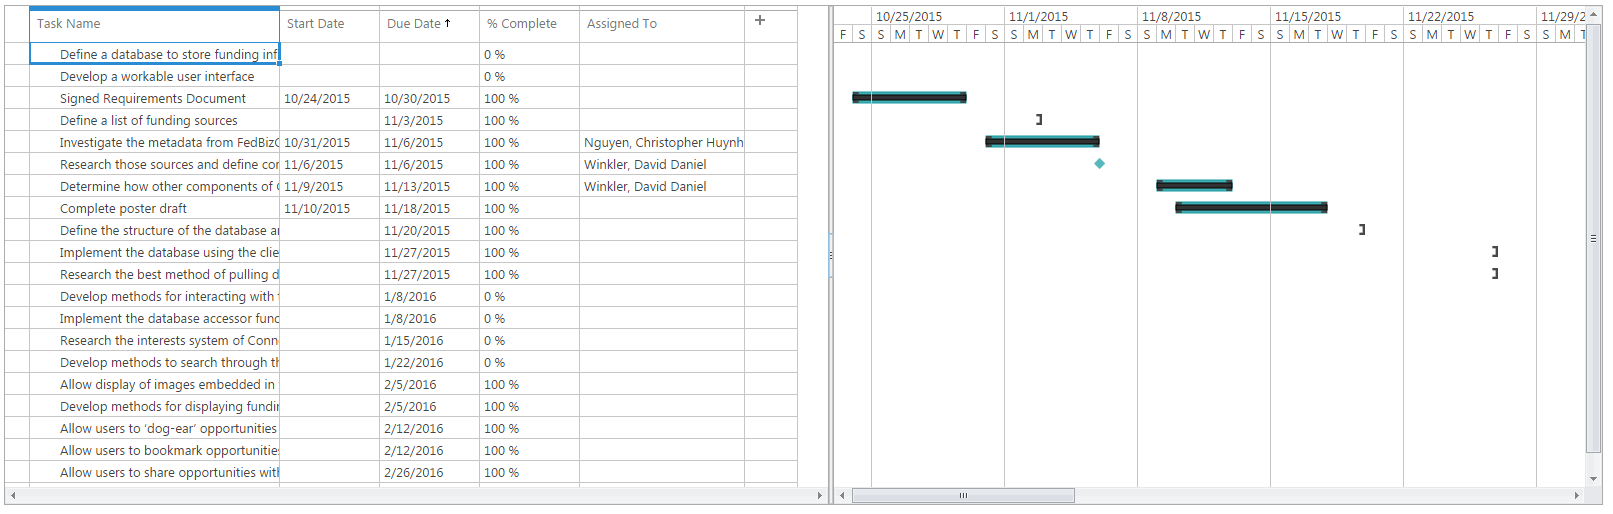
\includegraphics[width=0.8\textwidth]{gantt.png}
    \caption{Our original Gantt chart}
    \label{fig:gantt}
\end{figure}
%%%%%%%%%%%%%%%%%%%%%%%%%%%%%%%%%%%%%%%%%%%%%%%%%%%%%%%%%%%%%%%%%%%%%%%%%%%%%%%%

We began with investigating the funding sources and the data that would need to be stored. Once we had decided what to get and where to get it, we defined the database tables and the XML parsers that filled them. We developed the user interface alongside the database and parsers to check our data. We essentially copied the Publications component's html, templates, and JavaScript and changed elements of the design as necessary.  

When it came time to implement the interest matching system our clients had asked us to do, they told us that they would handle that part, because they have their own pattern matching system. So, a large part of our work was taken care of, and we started work on extra things our clients asked for. 

\subsection{Requirements Changes}

\begin{tabularx}{\textwidth}{|c|X|X|X|}
    \textbf{Number} & \textbf{Requirement} & \textbf{What happened to it}  & \textbf{Comments}\\
    \hline
    1.a & Investigate the metadata from FedBizOpps.gov and Grants.gov to determine how best to extract data from them. & After investigating those funding sources, we learned they publish their opportunities in XML files. We decided to write XML parsers to populate our database. \\
    \hline
    1.b & Define a list of funding sources & Our clients told us to focus on Grants.gov and FedBizOpps.gov, so we did not spend much time researching alternatives. \\
    \hline
    1.c & Research those sources and define common attributes to be stored & We created a list of attributes that would need to be stored, and translated those into a database design. \\
    \hline
    1.d & Determine how other components of Connected to Research will interact with the funding component & Other components can interact with the Funding component through a set of scripts we've created. & Each component has a different functionality intended by our client. Depending on the job of the other component, another groups' work could find our scripts helpful or not. \\
    \hline
    1.e & Define the structure of the database and develop a database schema & After defining the attributes to be stored, we translated them into a database design. \\
    \hline
    1.f & Research the best method of pulling data from funding sources & After finding the funding sources' XML sources,we chose to use those. \\
    \hline
\end{tabularx}
\begin{tabularx}{\textwidth}{|c|X|X|X|}
    1.g & There may need to be multiple ways of pulling information & There are weekly and nightly files from FedBizOpps, and we chose to focus more on the weekly file. & As forGrants.govXML files, they contained all their funding opportunities. \\
    \hline
    1.h & Implement the database using the client's preferred database system & The previous team's implementation of the Publications component usedMySQL, so we extended their work. \\
    \hline
    1.i & Implement the database accessor functions using the client's preferred language (Because the component will need to be integrated with other components) & The client asked us to use PHP on the back-end, and JavaScript on the front-end. \\
    \hline
    2.a & Research the interests system of Connected to Research to determine how to apply interests to funding opportunities & As mentioned, the client asked us not to do this. \\
    \hline
    2.b & Develop methods to search through the database and retrieve results related to the associated interest & Same as above. \\
    \hline
    3.a & Develop methods for displaying funding opportunities to the user, as shown in mockups by the previous team & Due to data deficiency, we couldn't match their mockups exactly. However, we got close. & See the Appendix for image comparison between the mockup and our end result. TODO: Add appendix number? \\
    \hline
    3.b & Allow display of images embedded in the opportunity description & We completed this task. \\
    \hline
    3.c & Allow users to bookmark opportunities and display them in a chronological list & We completed this task. \\
    \hline
    3.d & Allow users to dog-ear opportunities for later review & We completed this task. \\
    \hline
    3.e & Allow users to share opportunities with other researchers through the site and through email & We completed this task. \\
    \hline
\end{tabularx}

\subsection{Original Design Document}
Not much changed between our design document and our implementation. The most obvious difference is in the interest tagging system. While we were prepared to tackle that challenge, we asked our clients how we should go about it. However, they told us that they didn't want us to do that, because they had their own, more sophisticated pattern matching system, and they didn't want us wasting our time on our own. 

The user interface also changed slightly. We removed the ability to sort the funding opportunities, and instead list all opportunities in chronological order based on expiration date. We also implemented the ability to toggle multiple search categories. 

We also didn't implement a page for the user's preferences and options, because we didn't need to work on preferences or interests. 

The database and back-end remain mostly the same as our design document describes it. The ERD also matches our final implementation.

%%%%%%%%%%%%%%%%%%  DESIGN DOCUMENT  %%%%%%%%%%%%%%%%%%%%%%%%%%%%%%%%%%%%%%%%%%%
\clearpage
\addtocounter{page}{9}
%%%%%%%%%%%%%%%%%%%%%%%%%%%%%%%%%%%%%%%%%%%%%%%%%%%%%%%%%%%%%%%%%%%%%%%%%%%%%%%%

\subsection{Original Tech Review Document}

For pulling the data from the funding sources, we were going to use the FBOpen API, developed by 18f. Instead, we chose to use the XML parsing approach. We chose not to use FBOpen because we didn't want to depend on an outside source for our project. XML parsing is simple enough that we could make our own system that works well for our purposes. 

For the database, we chose to use MySQL instead of PostgreSQL, because the previous Publications component of the project was already using MySQL. 

To develop the user interface, we continued to use bootstrap, because the rest of the project uses bootstrap.  We also continued using PHP and JavaScript, because the rest of the project also used those languages. 

%%%%%%%%%%%%%%%%%%  TECH REVIEW DOCUMENT  %%%%%%%%%%%%%%%%%%%%%%%%%%%%%%%%%%%%%%
\clearpage
\addtocounter{page}{10}
%%%%%%%%%%%%%%%%%%%%%%%%%%%%%%%%%%%%%%%%%%%%%%%%%%%%%%%%%%%%%%%%%%%%%%%%%%%%%%%%

\section{Poster}
%%%%%%%%%%%%%%%%%%  POSTER  %%%%%%%%%%%%%%%%%%%%%%%%%%%%%%%%%%%%%%%%%%%%%%%%%%%%
\clearpage
\addtocounter{page}{1}
%%%%%%%%%%%%%%%%%%%%%%%%%%%%%%%%%%%%%%%%%%%%%%%%%%%%%%%%%%%%%%%%%%%%%%%%%%%%%%%%

\section{Blog Posts}
During the first quarter, we made regular blog posts. During the second quarter and beyond, we often forgot to log our work.

% IEEEtran is retarded so we can't fit all of the blog posts in one section.
% It counts alphanumberically (a,b,c...), and we have more subsections than
% there there are letters.
\subsection{October Posts}
\subsubsection{Tuesday (October 6, 2015)} \hspace*{\fill} \\
    \textbf{What We Did: }
    On this day, CS 461's lecture ended earlier than usual because each group had found their group members. Our group decided to find a place to meet right after and as our meeting progressed, we contacted our client via email for an official meeting with them. Our client was busy on that week's Thursday, which was October 8th. Instead, we decided to meet on Tuesday of the following week, October 13.  
    
    \textbf{How We Did It: } 
    We met after class and got to greet each other as to learn each member's background in Computer Science. We initiated contact by sending an email in an attempt to learn each other's schedules and make a meeting. We learned that their schedules favored meeting at 4pm, Tuesdays and Thursdays.  
    
    \textbf{Problems We Encountered: } 
    During our initial team meeting, we learned that none of us were very confident in our web development skills. However, after discussing it, we discovered that our skills and interests complement each other well. We decided that each of us would focus on a component of the final design, and improve our skills as necessary to aid our other team members. We would collaborate and specialize as necessary to complete our goals.  

\subsubsection{Tuesday (October 13, 2015)} \hspace*{\fill} \\
    \textbf{What We Did: }
    This was our first official group meeting with our client. Since our clients are stationed in Washington, our only way of communication was either by phone, email or skype. For this meeting, our method of communication was through skype so that our clients can get a recognition of our face to names. During the meeting, we each introduced ourselves by answering a set of questions provided by our clients. The clients wanted to get a better view of us as developers and discover our skills. We also discussed what requirements the clients desired and how we could meet them.  

    We also met with our teaching assistant, Jon Dodge. We didn't have much to report, but he gave a summary on what he expected from us.  
    
    \textbf{How We Did It: } 
    We emailed our client last week to schedule a meeting with them officially and we kept in contact with each other via email. Our client had sent us a Skype Invitation via email prior to the meeting and one of our team members used his laptop as the main communication channel. Since it would be confusing and separated if we each used our own laptop to talk with our client.  
    
    \textbf{Problems We Encountered: } 
    Shortly after meeting with the clients, we discussed the technologies we were asked to use, and how to implement them. We agreed that pulling data from the funding sources is the primary source of difficulty in our project.  

    Initially, the client asked us to look at the metadata related to the funding source websites. Our initial investigation involved looking at the HTML itself and identifying the HTML tags that correspond to the entries we were interested in. After we had done this, we developed our initial design for extracting data. We didn't pursue this approach for very long, however.  

\subsubsection{Saturday (October 24, 2015)} \hspace*{\fill} \\  
    \textbf{What We Did: }
    We started outlining the requirements document after our meeting with our teaching assistant Jon Dodge earlier in the week on Tuesday. We used our earlier meeting with the client to brainstorm rough requirements. The clients emailed us some work from the previous team, and we used that for further insight into what they wanted. We scheduled a meeting with our clients for the next Tuesday.  
    
    \textbf{How We Did It: } 
    Our clients required us to use four technologies in our implementation. The first type of technology required was methods of retrieving data in order to pull data from funding opportunities sources. The second type of technology required was database systems to store data from either the user or the funding opportunities sources. The third type of technology required was methods of the presenting the data to display funding opportunities for the user to view. The fourth and last type of technology required were computer languages used for manipulating aggregated data.  
    
    \textbf{Problems We Encountered: } 
    After our meeting, we decided that our first idea (HTML scraping) would be very inefficient. This approach would involve figuring out some way to iterate through all of the pages of each funding source website. Then, we would need to download the raw HTML of the website and parse through it, searching for tags corresponding to the fields we identify. If we had implemented this approach, we could have likely run into problems later on if the funding source had decided to redesign their website in any way. It also would have been very slow, with a large amount of overhead for the data gained. We would need to download a large amount of HTML files. We would have to parse through a lot of irrelevant  

    HTML tags until we find one that corresponds to a tracked field in our database. This would be very time- and space-inefficient. We unanimously decided that this was the wrong approach to take for the design.  

\subsubsection{Tuesday (October 27, 2015)} \hspace*{\fill} \\  
    \textbf{What We Did: }
    For this day, we had our second group meeting with our client via Skype regarding what they want for the requirements document. During the meeting, we asked our clients some questions to clarify the concept that they had in mind, so that we know what requirements to include. We met to discuss the implementation of our data parsing component. During the meeting, we took notes on the technologies and specific requirements they had. After the meeting, they emailed us a bulleted list of requirements.  

    Our clients also outlined the specific technologies we would need to use. They asked us to use PHP for the back-end scripting, JavaScript for the front-end, and PostgreSQL for the database. We later used this information of our Tech Document.  

    We translated the bulleted list the client gave us into a set of requirements, and broke them down into smaller, simpler instructions. We also added more requirements based on what they had told us during our meetings but had glossed over in their list. We felt it was better to add these to our requirements instead of leaving them in the air as to whether we would implement them or not. We didn't want to disappoint our client.  
    
    \textbf{How We Did It: } 
    Similar to our first Skype meeting with our client, they had sent us an invitation where we could join them by just having one member click the invitation and log into Skype. Prior to the meeting, we had already brainstormed some questions for our client that required clarification.  

    Our client asked us to use certain technologies, but we decided not to list the technologies in our requirements document. Our client told us we could be flexible in where to use them, and didn't seem dead-set on us using them. They accepted that we left it off the document and signed it as-is. Later, we mentioned the technology requirements in our Technology review assignment.  
    
    \textbf{Problems We Encountered: } 
    During our meeting, our clients gave us a small set of requirements that we needed to think about more thoroughly. We needed to work with them to discover more intricate requirements and break their relatively vague requirements into a concrete set of instructions for us to implement.  

    The client wanted us to use PostgreSQL, but we are not sure how to set up a development environment that we all can access that will allow us to test with a PostgreSQL database. We know that we have access to our personal MySQL servers through the university, but we are not sure what sort of effort will be required for converting between MySQL and PostgreSQL. We ultimately decided to test our code locally. When we get to implementation, we will need to discuss specifics of how to accomplish this.  

\subsubsection{Thursday (October 29, 2015)} \hspace*{\fill} \\  
    \textbf{What We Did: }
    We met on this day to discuss and create the timeline we expect to complete during the whole year of the senior design course. In order to create the timeline, we used a Gantt Chart to organize the different tasks that we had thought of. The Gantt Chart we created is included on our SharePoint site, so we could keep track of the tasks we have completed so far. We also improved the formatting and completed the requirements document in order to meet the due date.  
    
    \textbf{How We Did It: } 
    In order to create our timeline we used SharePoint to create a Gantt Chart by listing the tasks that we would need to follow through based on what our requirements document stated. The deadlines for completing each task was more of an estimate which we thought would be feasible. It was not meant to be a concrete requirement.  
    
    \textbf{Problems We Encountered: } 
    As part of our ongoing research, we came across other methods of pulling metadata from the sources. A helpful Google search found us the full FedBizOpps.gov XML dump. After looking into it further, we found more information about the XML files published by Grants.gov and FedBizOpps.gov, thanks to 18f. 18f is a US government agency that makes digital products for government organizations. They created their own scripts for parsing the XML data published by both our targeted funding sources. 18f's XML parser is named FBOpen, and is released under the public domain. This is good for us, because it means we can adopt their code and adapt it for our specific uses when necessary.  

\subsubsection{Friday (October 30, 2015)} \hspace*{\fill} \\  
    \textbf{What We Did: }
    To summarize this week's progress, we focused a lot on completing the requirements document and getting it approved and signed by our client. So we planned the work that would need to be done. We met up earlier this Tuesday with our client. It is safe to say that we turned in our final requirements document approved and signed by our client and our group.  
    
    \textbf{How We Did It: } 
    For us to finish and complete the requirements document on time, we had to be on topic each time we had a meeting because our schedules differed and didn't allow us to meet as much per week. By being productive for the week of October 26, we each delegated different portions of the requirements document to each member. Then as we added more details for the document, each of us had proofread over each other's writing and from time to time, we had to make changes. It was more efficient for our team to use this methodology because we could ask each other to elaborate on what they wanted to say and at the same time critique each other's work. By questioning each member's idea, we were able to see different viewpoints and potential improvement on our methods.  
    
    \textbf{Problems We Encountered: } 
    We were not sure how much information to include on the requirements document. We spent a lot of time looking it over as a group, and asked the client if they were satisfied. They were, and signed it.  

\subsection{November Posts}
\subsubsection{Friday (November 6, 2015)} \hspace*{\fill} \\  
    \textbf{What We Did: }
    This blog post is to highlight the week's earlier Tuesday, where we had our weekly meeting with our Teacher Assistant to clarify some questions we were unsure of. On the same Tuesday, we sat down together as a group to brainstorm how we would like to present the different types of technologies we will use for the project. We also delegated responsibilities for each member of the team to the completion of the document. Similar to the requirements document, each member volunteered to finish one category of technology.  
    
    \textbf{How We Did It: } 
    Our method of brainstorming the different technologies that may be utilized in the project was to research alternative technologies that would help reach our main goals. We defined our main goals as the different technological methods that we would implement in order to complete the funding component. These technological methods were defined in the technology review document.  
    
    \textbf{Problems We Encountered: } 
    While researching the FBOpen technology, we discovered that it is implemented with JavaScript. However, our client has asked us to use PHP on the backend. Because the XML parsing is a back-end process, this would conflict with our client's request. After discussing it, we decided it might be better to implement the back-end XML parsing scripts ourselves, using the FBOpen implementation as a reference for the structure of the XML documents we are using.  

\subsubsection{Tuesday (November 10, 2015)} \hspace*{\fill} \\  
    \textbf{What We Did: }
    On this day, we had finished our Technology Review document by reviewing what we already had and adding more information. As a group, we also discussed the possible technologies and what the feasibility would be like if we were to use them for our project. Feasibility is an important part of the project because we want to be able to meet our deadlines and be able to complete most of the functionality of the funding component. We do not want to waste time looking into technologies that we may or may not use.  
    
    \textbf{How We Did It: } 
    Our process to complete the technology review document was to research the alternative methods to compare and contrast it with our main technology methods. During the research, we would summarize our findings and determine the best solution for the project.  
    
    \textbf{Problems We Encountered: } 
    In researching the XML parsing, we decided as a group that we would look into implementing it ourselves. This will involve more work on our end, but ultimately more maintainable. Instead of relying on outside tool that we may need to configure to suit our purposes, we can design our own tailor-made scripts. This will give us greater control over, and understanding of, our system. Implementing it ourselves also means that we (and likely our successors) will not need to worry about updating the FBOpen scripts and integrating the changes into our code.  

\subsubsection{Friday (November 13, 2015)} \hspace*{\fill} \\  
    \textbf{What We Did: }
    For this week's summary, we fleshed out our plan's for the website's design with additional details. We also researched the different approaches we could use to implement the website. Also we have become familiar with the different technologies that we will be using to construct the funding component. Then we discussed the design of the database furthermore and created a document to show the data we believe should be stored in the database. We have also identified the similarities between the data that would be stored.  
    
    We had done research on the XML documents published by the funding sources before, and created three sheets within it to describe the data contained for each funding source. We listed the fields associated with each source, any notes, and related fields between them. Then, we created a super sheet for the shared attributes between them. We used this to create an overview for our database tables.  
    
    \textbf{How We Did It: } 
    Within the group meetings, we had discussions regarding how we would like the database to interact with the display of information on the website and how the back-end manipulates the many files of data. We would discuss what each of us thinks on the approach and then we would state alternatives and how we could improve the design.  

\subsubsection{Monday (November 16, 2015)} \hspace*{\fill} \\  
    \textbf{What We Did: }
    On November 16th, we had finished the rough draft expo poster for our group.  
    
    \textbf{How We Did It: } 
    We utilized the Power-point template that was provided to us in order to keep consistency with the branding guidelines for OSU. To start the poster, we laid out a skeleton of what we wanted and where on the poster. Then we filled in the sections with relevant information while following guidelines provided to us. We had to think as a team, what the audience would like to see on presented on the poster and what type of audiences we might get at the engineering expo. Therefore, revisions were made in order to refine our rough draft. There is most likely going to be more revisions as the year goes on.  
    
    \textbf{Problems We Encountered: } 
    There was more information that we wish we could have included on the poster, but since space was limited, we only picked what was relevant and important to the audience. We also could not include much information about implementation, which made describing the final product difficult.  

\subsubsection{Friday (November 20, 2015)} \hspace*{\fill} \\  
    \textbf{What We Did: }
    The weekly update for November 16th week was we met to discuss our poster, our elevator pitch and any upcoming assignments. On Monday, we finished our poster and posted it on our SharePoint along with the website's documents. We were unsure as to how much we needed on our poster but we gave it a good overview of the project. Then we started on the script of our elevator pitch and went through a few different approaches in order to memorize the contents. Lastly, we discussed the upcoming assignments and when we can meet in order to complete them. Our minds needed to be collective on one design that will work.  
    
    \textbf{How We Did It: } 
    Since the poster process is already explained above, we can now explain our process for our elevator pitch. To start off, we went through our previous documents to see where we could highlight some of the important points in our project. Next we created a skeleton of our elevator pitch. Then we filled it with contents and decided to read it out loud with a timer. We were definitely over the 30 second time limit. So we broke up the elevator pitch into three different sections, according to the number of members in our group. As we progressed, we kept rearranging the sentences without changing the meaning of what we would like to convey. After many iterations and trials, we came to a concluding elevator pitch that was within the 30 second time limit.  
    
    \textbf{Problems We Encountered: } 
    Some problems we encountered were during the different trials of the elevator pitch, sometimes the team members would mess up and sometimes we would forget our parts. It was a frustrating process, but nonetheless to solve our issues, we had each member type out the format of how they usually speak. Only changing the sentence formatting and yet keeping the meaning the same.  

\subsubsection{Friday (November 27, 2015)} \hspace*{\fill} \\  
    \textbf{What We Did: }
    This week was short but we started outlining the design document and planned to keep working on it by setting up upcoming meetings. We decided to meet during dead week in order to complete the progress report as well as continuing on the completion of the design document. Due to thanksgiving, we couldn't meet in person or online.  
    
    \textbf{How We Did It: } 
    Since this week we couldn't meet up as much as the other weeks, we tried to work as much as possible on the design document and then possibly add more remotely during the Thanksgiving break. Before the break, we had a skeleton for how we would like to layout the design document sections. Then we started to fill in information we already knew into sections we were familiar with.  
    
    \textbf{Problems We Encountered: } 
    At first it was hard to know what information we needed to include in the design document, but after some researching we learned what was essential to add to the document while keeping with the IEEE format. Also, asking the Teacher Assistant for clarifications of what we should include was very helpful.  

\subsection{December Posts}
\subsubsection{Wednesday (December 2, 2015)} \hspace*{\fill} \\  
    \textbf{What We Did: }
    Our final fall term meeting with our Teacher Assistant was yesterday (Tuesday, December 1). Then we met up afterwards to complete more of the design document and we got a majority of it completed. By the end of the day, we had completed our design document.  
    
    \textbf{How We Did It: } 
    For the meeting on Tuesday, we continued developing on what we already had for our design document. As we each proofread what each member had wrote, it jogged better improvements on our document. We applied the newer changes and continued to research what our document was missing. As for Wednesday's meeting, most of the workflow was the same as Tuesday but we were closer to completing the design document itself. When we completed the document, we sent the final copy to our Teacher Assistant, as to double check what we were still missing.  
    
    \textbf{Problems We Encountered: } 
    Our major problems was in not understanding the IEEE format required for a Software Design Document. We each read through the document, and weren't sure whether we needed to include a bulleted list of every design viewpoint, or if we needed to simply address them at some point in a document of our own layout. We looked online for examples of other design documents, and found that it was better to include general sections, and having many complex UML diagrams was unnecessary. Instead, we included one ER diagram to describe the layout of our database, which we feel is part of our design most likely to confuse readers. After we finished, we emailed our Teaching Assistant to get his opinion on the document, and after getting his approval, we saved the document as a PDF to our documents section of the SharePoint site.  
    
    During the creation of our document, we were not sure how to represent the database. We had thought about the interest tagging system, but had not designed a database table to represent them. We discussed a couple approaches, but there were confusing difficulties that we weren't sure how to work around. They are described in the Design Document. There are different fields used to categorize opportunities between Grants.gov and FedBizOpps.gov. These can be CFDA numbers, categories, Classification codes, and NAICS codes. Each of these could be associated with a different interest held by a user. We would need some way of storing all of those possible values with each interest. The design we came up with was to store a list of strings for each interest code/category/etc.  

\subsubsection{Friday (December 4, 2015)} \hspace*{\fill} \\  
    \textbf{What We Did: }
    This is our weekly update for week 10. We met up more this week in order to finish the last two documents for our project. As we completed the design document, we immediately started to work on the progress report. By Friday, we had already completed both documents.  
    
    \textbf{How We Did It: } 
    We were more productive during each meeting for this week, more than usual because we wanted to meet the upcoming deadlines and not fall behind. As we sent out our final copy of the design document to our Teacher Assistant, we started to work on collecting the blogs together and describing more in-depth of what had happened. We also looked into what we could possibly include in our progress report as to be more detailed on our development.  

\subsection{January Posts}
\subsubsection{Thursday (January 7, 2016)  }
    \textbf{What We Did: }
    Started on the project and tried to get connection.php to work with our own database. We are not sure how to use the scripts running with our database.  
    
    \textbf{How We Did It: } 
    We tried different methods to jumpstart on the project.  
    
    \textbf{Problems We Encountered: } 
    We were not sure how to get the scripts to run with our own database.  

\subsubsection{Tuesday (January 12, 2016)} \hspace*{\fill} \\
    \textbf{What We Did: }
    We continued where we left off from the last meeting. We also started to work on the XML parsing, XML downloading, and debugging Javascript errors.  
    
    \textbf{How We Did It: } 
    We delegated the work among the three of us so that we all wouldn't be stuck on one single problem.  
    
    \textbf{Problems We Encountered: } 
    There was a ng-repeat duplicates Javascript error that we found and was trying to fix it so that we could display the front-end displays.    

\subsubsection{Monday (January 18, 2016) David's Work  } \hspace*{\fill} \\
    \textbf{What He Did: } 
    He finished the XML download scripts and updated the database creation script.  
    
	\textbf{How He Did It: }
	There are PHP functions to download the weekly and nightly FBO files, and the Grants.gov full XML. The FBO weekly file and Grants file are large and take a long time to download. As for the database creation script, it creates tables for storing the funding opportunity data. The tables are as described in the Design Document, in the documents section.   
    
	\textbf{Problems He Encountered: }
	There were some irregularities in the XML files that he had to discover on his own. 

\subsubsection{Tuesday (January 19, 2016) Chris's Work  } \hspace*{\fill} \\
    \textbf{What He Did: } Completed and tested a basic XML parser that parses elements in the XML file.   
    
	\textbf{How He Did It: }
	The elements in the XML parser are placed into their respected grant objects which are structures. Then all of the objects are appended onto an array. The code is easily scalable for more elements if needed. The array is to make the implementation for our SQL insertion easier.   

\subsubsection{Tuesday (January 19, 2016) Benny's Work  } \hspace*{\fill} \\
    \textbf{What He Did: } 
    Tried to get rid of the AngularJS error of ng-repeat duplicates.  
    
	\textbf{How He Did It: }
	Tested the track by method in the ng-repeat directive to see if it debugs the error, but no viable result. Tried to email client to see if they are getting any thing to show up on their screen.  
    
	\textbf{Problems He Encountered: }
	Still getting the same error and no display on publications page.  

\subsubsection{Monday (January 25, 2016) David's Work  } \hspace*{\fill} \\
    \textbf{What He Did: } 
    Finished FBO nightly parser.  
    
	\textbf{How He Did It: }
	Since the nightly files are not XML, he could not parse them as normal XML like the weekly FBO and daily Grants.gov XML files. Up to this point, the only notice types that are added to the database are pre solicitation, sources sought, combined synopsis/solicitation, and special notice. 

\subsubsection{Monday (January 25, 2016) Client Meeting  } \hspace*{\fill} \\
    \textbf{What We Did: } 
    We met with the client to give them an update on the progress we've made. We told them the work we've done and what we expect to do soon. They also gave more detail on how they expected our design to look, including filter options and information display. We also discussed the types of notice that should be taken from FedBizOpps. 

\subsubsection{Thursday (January 28, 2016) Benny's Work  } \hspace*{\fill} \\
    \textbf{What He Did: } 
    Created a funding.html for the user to view the funding opportunities and a funding.js file to manage the funding module, controllers and directives. Also added a filter.tpl.html to format the filtering column on the main HTML page.  
    
	\textbf{How He Did It: }
	Created a simple format of funding.html using bootstrap and simple Javascript file for manipulating funding controllers. Linked the index.html to the funding.html page and vice versa. 
    
	\textbf{Problems He Encountered: }
	There is an implementation error in the filter-funding.php file that will be fixed. 

\subsubsection{Friday (January 29, 2016) Chris's Work  } \hspace*{\fill} \\
    \textbf{What He Did: } 
    Started the basis of the parser to work for Grants.gov files. Ideally, will create a test for larger XML files from Grants.gov. Started working on the SQL insertion part of the parser. 
    
	\textbf{How He Did It: }
	Created a foundation of idea of how the Grants parser will work with small XML data. 
    
	\textbf{Problems He Encountered: }
	Small kinks still needed to be worked out in the code for full functionality. 

\subsection{February Posts}
\subsubsection{Thursday (February 4, 2016) David's Work  } \hspace*{\fill} \\
    \textbf{What He Did: } 
    Finished the FBO nightly file parser which adds records that aren't in the database and updates for AMDCSS and MOD notice types. Also finished the FBO weekly file parser which adds and updates records in our database. 
    
	\textbf{How He Did It: }
	The parsers read through all of the records in the XML file one by one, adding each record or updating existing records. The assumption here is that the weekly file takes precedence over anything else. So if a record in the XML file contradicts a record in our database, our record will be overwritten. 
    
	\textbf{Problems He Encountered: }
	Some of the records are odd and don't have solution numbers. While others have strange date formats, and the descriptions have HTML tags in them. The script rejects records with no solution numbers and ignores improper dates. 

\subsubsection{Friday (February 5, 2016) Benny's Work  } \hspace*{\fill} \\
    \textbf{What He Did: } 
    Still working on filter-funding.php script at this point. Also worked on funding.js to get the main funding opportunities column started.  
    
	\textbf{How He Did It: }
	Created a template view for the main column with bootstrap and certain tags and fields are subject to change depending on changes made to filter-funding.php script. Created a new directive and a controller for funding items to appear in the main column.  
    
	\textbf{Problems He Encountered: }
	There are still some potential bugs in filter-funding.php script that will need to be worked out.  

\subsubsection{Monday (February 8, 2016) Chris's Work  } \hspace*{\fill} \\
    \textbf{What He Did: } 
    Finished the insertion of opportunities from Grants.gov. 
    
	\textbf{How He Did It: }
	Used SQL insertion method to insert the opportunities into the database. 
    
	\textbf{Problems He Encountered: }
	There are some minor problems that need to be fixed regards to memory and timeout limit. 

\subsubsection{Monday (February 15, 2016) (Post Midterm) Client Meeting  } \hspace*{\fill} \\
    \textbf{What We Did: }
    Today we met with our client and discussed what we already have for the Alpha level of the project. Our client is satisfied with what we already have and we have discussed what to add to the Beta level. We have already finished the Alpha level of the project by this point. 

\subsubsection{Friday (February 19, 2016) Chris's Work  } \hspace*{\fill} \\
    \textbf{What He Did: } 
    Fixed all shortcomings of the Grants parser. Currently learning how to use AngularJS more proficiently to work on the deadlines column.  
    
	\textbf{How He Did It: }
	He converted the parser's design to stream the data by iterating the structures rather than holding all of the input data into a buffer.  

\subsubsection{Friday (February 19, 2016) Benny's Work  } \hspace*{\fill} \\
    \textbf{What He Did: } 
    Worked on the funding deadlines column.  
    
	\textbf{How He Did It: }
	Added a funding-deadlines.php file to select the funding deadlines that pertain to the specific user and will need to fix the calculating of the time of deadline. Added a insert\_funding\_deadlines.php file to insert the funding deadlines into the new table called ctr\_user\_fund\_link. Added a template for displaying the funding deadlines called funding-deadlines.tpl.html. Added a new CSS style for the funding deadlines column. Added a new table to the database\_creation script for holding funding deadlines. 
    
	\textbf{Problems He Encountered: }
	There are some bugs in inserting the funding deadlines that will be addressed. 

\subsubsection{Friday (February 26, 2016) Benny's Work  } \hspace*{\fill} \\
    \textbf{What He Did: } 
    Worked on completing the add button feature that sends opportunity to the funding deadlines column when the user clicks on it. Refactored the SQL queries in the filter column so that it displays the count that is from the ctr\_user\_fund\_link table. Also the funding items main column is working properly now. Started to look into the multi-toggle filtering as the client requested. 
    
	\textbf{How He Did It: }
	Used components from bootstrap to add a button and AngularJS to bind that button with an insert SQL statement to add the specific funding opportunity to the deadlines column. 
    
	\textbf{Problems He Encountered: }
	There is only adding to the deadlines column, potentially might want to have a remove feature in the deadlines column. 

\subsection{March Posts}
\subsubsection{Saturday (March 5, 2016) Benny's Work  } \hspace*{\fill} \\
    \textbf{What He Did: } 
    Worked on fixing the type checking for the filter column groups Agency, Notice, Post Date, and Due Date. In the end we chose to utilize a second controller for the sharing feature so that it can be independent by each funding opportunity. 
    
	\textbf{How He Did It: }
	Tested the share funding button and then refined it accordingly. Tinkered with the sharing feature for quite a while, until we found that the functionality wasn't independent by each funding opportunity. 
    
	\textbf{Problems He Encountered: }
	At first we ran into the problem that the sharing feature was doing the same behavior for all opportunities and not unique enough. 

\subsubsection{Saturday (March 12, 2016) Benny's Work  } \hspace*{\fill} \\
    \textbf{What He Did: } 
    Finished up poster requirements with group for this term. Also worked on finishing up final video and final report. Also worked on getting the dog ear favorite to be feature complete. 
    
	\textbf{How He Did It: }
	Completed parts of the poster and rendered the final video for group. 

\subsection{April Posts}
\subsubsection{Wednesday (April 6, 2016) Benny's Work  } \hspace*{\fill} \\
    \textbf{What He Did: } 
    Met up with client for the second time of the term and discussed the upcoming plans and extra features. For development, added a peak feature that displays the top 3 recommended fundings for the index.html and funding.html.  
    
	\textbf{How He Did It: }
	Utilized some CSS and bootstrap to create a similar peak feature to the last group. The design of the peak feature requires to split the ng-app of funding.html and index.html, so that each page shows the other's top 3 items. 
    
	\textbf{Problems He Encountered: }
	Had a hard time finding a way to use two ng-apps in one HTML file. 

\subsubsection{Saturday (April 16, 2016) Benny's Work  } \hspace*{\fill} \\
    \textbf{What He Did: } 
    Met up with group to solve the bug of funding opportunities not displaying due to implementation of the new feature of multi-toggling. 
    
	\textbf{How He Did It: }
	Added console logs in Javascript file to find and figure out what the error is and how a fix can be applied. 
    
	\textbf{Problems He Encountered: }
	Still trying to figure out why multi-toggling feature is not working. 

\subsubsection{Friday (April 22, 2016) Chris's Work  } \hspace*{\fill} \\
    \textbf{What He Did: } 
    Met up with client and group to discuss current progress and demonstrating multi-toggle filter and other enhancements. Received feedback on our poster from our client where they would like changes to be made. Our group revised the poster, made the changes necessary, and sent it back for approval by client. 
    
	\textbf{How He Did It: }
	Revised the poster with group. Started working on getting agency logo images for each funding opportunity. 

\subsubsection{Friday (April 22, 2016) David's Work  } \hspace*{\fill} \\
    \textbf{What He Did: } 
    Added a script so developer can add images for agency logos to funding opportunities.  
    
	\textbf{How He Did It: }
	Created an img\_agency directory and an agency\_add\_image.php file to insert the images using an image URL and agency name. Last Wednesday, modified the funding-items.php script to add the image file name to the JSON returned when queried. 

\subsubsection{Sunday (April 24, 2016) Benny's Work  } \hspace*{\fill} \\
    \textbf{What He Did: } 
    Created a front-end for displaying the agency images. 
    
	\textbf{How He Did It: }
	Grabbed the image queried by David's funding-items.php script to display the image with the help of AngularJS. 
    
	\textbf{Problems He Encountered: }
	At first the images didn't display, but after a while of figuring out with Chris, we utilized ng-show from AngularJS to complete the agency image display. 

\subsubsection{Friday (April 29, 2016) Benny's Work  } \hspace*{\fill} \\
    \textbf{What He Did: } 
    Slowed down on development because most of the client's requests are fulfilled and started to work on the poster to get approval from T.A. and client. 
    
	\textbf{How He Did It: }
	Revised poster even more for the preparation of Expo. Also worked on midterm report and video. 

\subsection{May Posts}
\subsubsection{Thursday (May 26, 2016) Benny's Work  } \hspace*{\fill} \\
    \textbf{What He Did: } 
    Added a script to populate user 2 with funding opportunities pertaining to the user in preparation for Engineering Expo. 
    
	\textbf{How He Did It: }
	Created a replication of David's script, researched and added NACIS codes for chemist (user 2) to the new script. Ran the script to populate user 2. 

\section{Final Poster}
%%%%%%%%%%%%%%%%%%  POSTER  %%%%%%%%%%%%%%%%%%%%%%%%%%%%%%%%%%%%%%%%%%%%%%%%%%%%
\clearpage
\addtocounter{page}{1} % should only be 1 page.
%%%%%%%%%%%%%%%%%%%%%%%%%%%%%%%%%%%%%%%%%%%%%%%%%%%%%%%%%%%%%%%%%%%%%%%%%%%%%%%%

\section{Technical Instructions}
\subsection{Visual Structure}
The website currently displays three columns, each with a designated role. The left-most column acts as a sort-by filter, where the user may select which funding opportunities he or she would like to view. In the middle column is the main view of the funding opportunities, whose display is based on the left-side column filter. Lastly, the right-most column is planned to be a collection of the research events and deadlines currently and upcoming. All of these are contained in the funding.html file. Figure \ref{fig:filter} shows the filter on the left of the page, and an opportunity on the right. The top of the image shows the navbar, with the logged-in user's name and profile picture.  

\begin{figure}
    \centering
    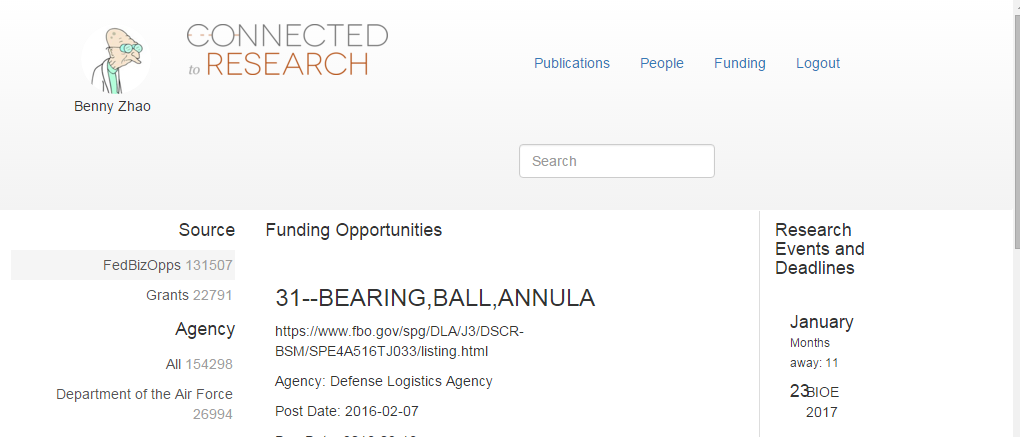
\includegraphics[width=0.8\textwidth]{filter.png}
    \caption{The funding page, showing filter and an opportunity}
    \label{fig:filter}
\end{figure}

Next, we have a funding.js file that basically acts as a link between the Ajax PHP scripts and tpl.html files. Within the funding.js file are AngularJS directives and controllers that manipulate what the user views in funding.html. The directives that are currently in the JavaScript file are for the navigation bar, the filtering column, the funding item column, and the deadlines column. The directives are for creating custom html tags that can grab information from the .tpl.html files. Then we have the AngularJS controllers that hold JavaScript functions and grabs functionality from the Ajax PHP files in the Ajax directory. 

\subsection{Technical Structure}
The funding component of Connected to Research is made up of three interrelated design entities. There is a front-end interface for users to interact with, a database storing all of the data related to funding opportunities, and a back-end suite of scripts to connect the front and back-ends. The web app allows users to create an account, be linked to funding opportunities, and interact with the opportunities by favoriting, sharing, and tracking them.  

The front-end of the application will be what users see and use to interact with the funding opportunities. It includes a browsing page with a multi-toggling filter panel. The togglable filter panel will allow users to intelligently refine the opportunities they see. They can toggle based on offering agency or offer type. 

The database is where the funding opportunity data is stored after being parsed out of the funding source's published data. It is populated by scripts existing in the back-end. 

The back-end is responsible for populating the database and retrieving data for the front-end. The funding opportunities are pulled from XML files made available by the funding opportunity sources and inserted into the database. The back-end also includes scripts to retrieve data from the database to serve the front-end. 

\subsection{Installation \& Use}
\subsubsection{Installation}
First, you'll need to git clone the repo somewhere internet-accessible. We used the public\_html directories on the schools servers. Those are accessible at http://web.engr.oregonstate.edu/~ONIDUSERNAME. You will also need to set up a MySQL server. We used the database provided by the school, though ONID. To access it as a student, go to onid.orst.edu, log in to ONID, and click 'Web Database' in the left pane. Note the database name and password it generates for you. Next, modify the file 'connection.php' in the project's 'scripts' directory. Modify the dbhost, dbname, and dbuser variables. Create a new file named 'password.php', and use it only to create a variable named dbpass, your database password. Don't push that file to github.  

After that, the site should be ready. If you used the school servers to host the site, be sure to reset your web directory from your TEACH page, https://secure.engr.oregonstate.edu:8000/teach.php. Click the link 'Personal Web Tools' under 'Account Tools', and when the page loads, click 'Reset Web Directory'. If you don't reset the web directory, you will get a 403 forbidden error. According to engineering college support staff, "The way php runs in user home directories, relies on the files being owned solely by the user and assigned to the upg (user personal group)." After cloning from git, the files will probably not belong to you, so the files will not be accessible. 

If the project has been set up properly, you can now load a blank white page. To make things appear, you will need to add data to the database. 

There are no special hardware, operating system, or runtime requirements needed to run the software. To run the web application, only a working computer with a functional web browser is needed. 

To host the software, users will need a server to host a website and MySQL server. Specific hardware and operating system choices can be left to the user. 

\subsubsection{Use}
There are multiple scripts included in the project's scripts directory. They are described in more detail in the documentation section.  

First, run database\_creation.php to create the necessary database tables. This script should only need to be used once. If new tables are created, they should be created through this file, and not through a direct SQL query.  

After the tables have been created, populate them with the scripts from the parsing directory. Use parse\_fbo\_weekly.php and parse\_grants.php to parse both sources of funding opportunities. These will download two large XML files from the sources, so make sure there are no space limits. They also take a long time to run, so you may need to increase the PHP execution time limit. Our scripts increase the limit to one hour. 

Use recommend\_to\_user.php to connect users to funding opportunities. This script takes three HTML GET variables: 
\begin{itemize}
    \item Type --- either article or call, for the publications component, or funding for the funding      component. 
    \item Users --- a comma-separated list of users to be connected to the funding. 
    \item Ids --- a comma-separated list of funding opportunity ids that exist in the database. 
\end{itemize}

Alternatively, there are scripts insert\_recommendations.php and insert\_recommendations\_user2.php, which will automatically connect the accounts user1 and user2 with funding opportunities. To use this, run the insert\_users.php script to create the test users 1-3. 

After the user has been connected to their funding and publications data, there should be opportunities appearing on the funding page and publications page. The funding page will not have any agency images to appear next to funding opportunities. To add them, use the script agency\_add\_image.php, which takes these HTML GET variables: 
\begin{itemize}
    \item Image --- A URL for an agency image 
    \item Agency --- An agency name that exists in the database 
\end{itemize}
    
After images have been added to the site, they should appear next to the appropriate funding opportunities. 

\section{Documentation}

\subsection{Scripts Directory}
\subsubsection{agency\_add\_image.php}
This script downloads an image file from a URL, and adds it to the database to map an agency to an image. It takes these HTML GET variables: 
\begin{itemize}
    \item Image --- A URL for an agency image 
    \item Agency --- An agency name that exists in the database 
\end{itemize}    

\subsubsection{article\_likes.php}
This defines a PHP function, get\_likes(), which returns a count of all articles a user has liked. It's parameters are a user id and mysqli object. 

\subsubsection{connection.php}
This script is used at the top of all PHP files that need to use the MySQL server. It connects to the server named in the variables and uses a file named password.php, which stores the server password. 

\subsubsection{create\_endnote.php}
This script creates an endnote for the publications component. 

\subsubsection{database\_creation.php}
This script creates all the database tables necessary for the project to function. User tables, funding tables, etc. Doesn't take any arguments, and returns success or failure for each table. 

\subsubsection{delete\_funding\_deadlines.php}
This script removes a funding opportunity from the currently logged-in user's list of funding opportunity deadlines, the list that appears in the right panel of the funding page. It takes one HTML GET variable: 
\begin{itemize}
    \item  id --- the ID of the funding opportunity to remove. 
\end{itemize}   

\subsubsection{favorite\_article.php}
This script adds a favorite record to the database for the currently logged-in user. It takes one HTML GET variable: 
\begin{itemize}
    \item id --- the article ID to be favorited. 
\end{itemize}    

\subsubsection{favorite\_funding.php}
Same as favorite\_article.php, but for funding opportunities. Takes a HTML GET variable, which is the funding ID to favorite. 
\begin{itemize}
    \item id --- the ID of the funding opportunity to favorite. 
\end{itemize}    

\subsubsection{generate\_citation.php}
This script creates an string for an MLA citation of a given article. It takes one HTML GET variable: 
\begin{itemize}
    \item id --- the ID of the article to cite. 
\end{itemize}    

\subsubsection{get\_users.php}
This script returns all of the users that exist in the database, encoded in JSON. 

\subsubsection{get\_users\_funding.php}
This script gets the users for the funding components 'share' feature. 

\subsubsection{insert\_events\_and\_deadlines.php}
This script adds a link between a user and a research item, which is used for the publication component. The events and deadlines are listed on the right panel on the publications page. It takes one HTML GET variables: 
\begin{itemize}
    \item id --- The research ID 
\end{itemize}    

\subsubsection{insert\_funding\_deadlines.php}
Similar to insert\_events\_and\_deadlines.php, this script links users to funding opportunity deadlines to be displayed in the right panel of the funding page. It takes on HTML GET variables: 
\begin{itemize}
    \item id ---  the funding opportunity ID 
\end{itemize}    

\subsubsection{insert\_recommendation.php, insert\_recommendations\_user2.php}
These two scripts connect our test researchers to some funding opportunities, based on an array of NAICS codes. It takes no arguments, but requires either 'user1' or 'user2' to exist. 

\subsubsection{insert\_users.php}
This is another test script that adds test users user1, user2, and user3 to the database. 

\subsubsection{insert\_xml.php}
This is the script the publications component uses to populate its articles database. It takes a raw string of XML, and parses it. It takes two HTML GET variables. 
\begin{itemize}
    \item XML --- The string of XML 
    \item type --- The type of XML 
\end{itemize}    

\subsubsection{login.php}
This handles the site's login functionality. It takes two HTML POST variables. 
\begin{itemize}
    \item email --- the user's email. 
    \item password --- the user's password. 
\end{itemize}    


\subsubsection{logout.php}
This handles the site's logout functionality. It takes no variables. 

\subsubsection{password.php}
This is a file that we used to store the database password. We kept this in a separate, untracked file so we wouldn't push it to github. 

\subsubsection{recommend\_to\_user.php}
Adds a record to the table to connect a researcher to an article, call to research, or funding opportunity. This is the script used to create the "connections" in Connected to Research. It takes three HTML GET variables. 
\begin{itemize}
    \item type --- either article (for publications), call (for a call-to-research), or funding (for a funding opportunity). 
    \item users --- a comma-separated list of user IDs to be connected to the items. 
    \item id --- A comma-separated list of item IDs to be connected to the users. 
\end{itemize}    

\subsubsection{register.php}
Used to register a new user profile for the site. Takes four HTML POST variables. 
\begin{itemize}
    \item name\_f --- the user's first name. 
    \item name\_l --- the user's last name. 
    \item email --- the user's email address. 
    \item password --- the user's chosen password. 
\end{itemize}    

\subsubsection{share.php}
Used to share an article from the currently logged-in user to another user. Unlike the items added through recommend\_to\_user.php, these show up under a 'shared' table, instead of 'recommendations'. It takes three HTML GET variables.  
\begin{itemize}
    \item type --- either article or funding. 
    \item id --- the funding or article ID to be shared. 
    \item users --- a comma-separated list of users to share the item with. 
\end{itemize}    

\subsubsection{view\_favorite\_fundings.php}
Queries the database to get all of the favorited funding opportunities of the currently logged-in user. Takes no arguments. 

\subsubsection{view\_favorites.php}
Used to get the favorited articles of the currently logged-in user., similar to view\_favorite\_fundings.php. Also takes no arguments. 

\subsubsection{view\_share\_fundings.php}
Similar to vew\_favorite\_fundings.php, but instead gets all items shared with the current user. 

\subsubsection{XML\_download.php}
This script contains functions for the XML parsers to use to download the XML files. It contains three PHP functions that take no arguments. One downloads the FedBizOpps nightly XML, another gets the weekly FedBizOpps XML, and the third gets the Grants weekly XML. 
 
\subsection{AJAX Directory}
\subsubsection{filter-funding.php}
This file is for the funding component. It uses mySQL statements to select the count of each filter category, put them in arrays and display it using AngularJS with the help of keys named groupItem, amount, and filterName. 

\subsubsection{filter.php}
This file is for the publications component. It uses mySQL statements to select the count of each filter category, put them in arrays and display it using AngularJS with the help of keys named groupItem, amount, and filterName. 

\subsubsection{funding-deadlines.php}
This file uses a mySQL statement to get the funding deadlines stored in ctr\_funding\_base. Then it calculates the funding deadlines by converting the raw date data in the table and storing it into an array, where it then returns the converted date to JSON. 

\subsubsection{funding-items.php}
This file depends on what the user chooses in the multi-toggling filters. Depending on which filters are chosen will utilize certain mySQL statements for selecting information from the table. The queried data is then stored in an associative array and encoded into JSON.  

\subsubsection{nav-bar-fundings.php}
This file is called from funding.js to use a mySQL statement to select the top 3 funding opportunities from ctr\_funding\_base and display it using the peak feature in the top navigation. 

\subsubsection{nav-bar-publications.php}
This file is called from app.js to use a mySQL statement to select the top 3 publications from ctr\_article and display it using the peak feature in the top navigation. 

\subsubsection{participation.php}
This file is used for app.js to select the call for participations in the publications component.   

\subsubsection{publication-items.php}
This file uses a GET variable to grab the type of article the user has selected from the filter. Then uses a switch statement to query the data based on the filter selection. The data is put into an associative array and encoded as JSON. 

\subsubsection{research-events-deadlines.php}
This file uses a mySQL statement to get the research and event deadlines for the publications component. Then it calculates the funding deadlines by converting the raw date data in the table and storing it into an array, where it then returns the converted date to JSON. 

\subsubsection{user-nav-bar-info.php}
A file that uses a mySQL query to select the user's information from the ctr\_user table based on the SESSION variable of email. 
 
\subsection{ JS Directory }

\subsubsection{angular.min.js}
This is the minified version of angular.js. The file angular.js is the framework of AngularJS. 

\subsubsection{app.js}
This file is used as the controller of the publications component. It pulls data based on users' requests then displays the data onto the view and updates the data. The file pulls data by executing one or more PHP files. It connects directives for all of the template html files that are used for the publications component to the main view of the publications component. 

\subsubsection{App.min.js}
This is the minified version of app.js. 

\subsubsection{bootstrap.js}
This file is a framework for developing responsive, mobile first projects on the web. 

\subsubsection{Funding.js}
This file is used as the controller of the funding component. It pulls data based on users' requests then displays the data onto the view and updates the data. The file pulls data by executing one or more PHP files. It connects directives for all of the template html files that are used for the funding component to the main view of the funding component. 

\subsubsection{login.js}
This file contains the implementation of user registering and login. If the user registers a user, register.php will be invoked via login.js or if the user is logging in, login.php will be invoked via login.js. 

\subsubsection{login.min.js}
This is the minified version of login.js. 

\subsubsection{npm.js}
This file is the package manager for Javascript. 

\subsubsection{npm.min.js}
This is the minified version of npm.js. 

\subsubsection{ui-bootstrap-tpls-0.12.0.min.js}
This file allows Bootstrap to use directives from AngularJS. 

\section{Lessons Learned}

\subsection{Benny Zhao}
The technical information I learned from this project was the process of developing a web application from a low fidelity to a high fidelity proof of concept. I also learned how to use AngularJS to bind data from the server side and client side. Also with the help of my teammates, I gained valuable knowledge of XML parsing with the use of PHP scripts.  

The non-technical information I have learned is how to format a poster adhering to branding guidelines and presenting a project at an expo environment. 

From this project I have learned about the documentation process of a large scale project, how to meet the clients' initial needs, and the process of meeting deadlines. I also learned about the adaptive process it takes to fit the clients' changing requirements. 

As for project management, I have learned how delegation of group tasks is important for meeting deadlines in a timely manner. Plus communication is crucial for conveying design implementations correctly and the success of the project.  
I have learned how to work in a development team environment by collaborating ideas and discussing proof of concepts with group members. Also that group members can have different interpretations of clients' needs and this can be confusing during development. 
If I could do it all over differently, I would have tried to a design profile page for the end-user to keep track of their own information and perhaps try a more efficient way of implementing data queries for the project.  

\subsection{Chris Nguyen}
I learned how to work well with front- and back-end web development. PHP and AngularJS were new languages to me and now I am decently fluent in PHP and nearly fluent in AngularJS. I still have to search online for documentation on HTTP for implementations that are not basic.  

I learned how to communicate well with my teammates and how we can collaborate easily without a need for a leader. We each had distinct strengths for this project, but we all learned from each other. I learned how you can explain broken code to another person and can potentially find your bug or error. 

What I have learned from project work is that you have to stay consistent with the project in order to make progress. I learned how to get my work done in time along with my teammates in order to demo the work to our client. What I have learned the most from this project is working on documentation and the process of working with a client.  

For project management, we give each person tasks to complete and the expected date or deadline to get it done by. What I learned from this is that if we stay consistent as in completing our work load on time then the project goes smoothly. There was one occasion that we could not finish a task on time, so we ended up grouping together and worked on it. I found that working together at times could be slow, but if everyone is up to date and figuring out multiple solutions then we could finish our task quickly. Overall, working in teams was beneficial to me since I can see progress in other parts of the project as well as how it was implemented.  

If I had to do this project differently, I wouldn't because we spent a good amount of time thinking about the design then implementing it. We all worked hard to get the project done and fulfilled our client's expectations. Our goal was to satisfy our client's needs and we completed that objective. 

\subsection{David Winkler}
I learned a valuable lesson about teamwork. In a more technical sense, I learned far more about back-end web development. I became almost fluent in SQL syntax, and usually no longer need to consult documentation when programming in PHP or SQL. I learned how to carry on an existing project, learn the source code and design plans, and make meaningful improvements to it. I also learned how to recognize gaps in team knowledge and volunteer to fill the gap.  

I also became much more familiar with \LaTeX.

Due to the fact that this group had no specific leader, I learned how to communicate effectively with team members to make sure that everyone knew what needed to be done, and who was willing to work on it.  

If I had to do this project differently, I'm not sure if I would. I feel that we all did our best and tried to finish our project satisfactorily.  

\subsection{Reference Material}
Websites that were helpful were stackoverflow.com, jsfiddle.net, php.net, w3schools.com, and youtube.com with stackoverflow.com being the most helpful and youtube.com being the least helpful of the five websites.  

With stackoverflow.com, we were able to find many different solutions to many of the conflicts we had with our project which resulted in us fixing almost all the problems with stackoverflow.com. The website jsfiddle.net allowed us to play around with code to see how a feature of the project would be implemented and executed. This helped us fix some small bugs. Some of which were preventing the implementation of the code from executing the way we wanted. Both php.net and w3schools.com provided us with documentation about AngularJS, SQL, and PHP. The last website youtube.com was our last resort to finding any information that we can't find in the first four websites and provided us with tutorials to help us understand concepts in AngularJS, SQL, and PHP.  

Anton Igorevich Dovzhik, one of the members of last year's capstone team that worked on our project for the publication component helped us with populating data for the web application. He gave us instructions on how to create users and populate data for that user.  

\end{document}
